\documentclass[a4paper,12pt]{article} % тип документа

% report, book



%  Русский язык

\usepackage[T2A]{fontenc}			% кодировка
\usepackage[utf8]{inputenc}			% кодировка исходного текста
\usepackage[english,russian]{babel}	% локализация и переносы
\usepackage{graphicx}
\usepackage{tikz}
\graphicspath{{./}}
\DeclareGraphicsExtensions{.png,.jpg}


% Математика
\usepackage{amsmath,amsfonts,amssymb,amsthm,mathtools} 


\usepackage{wasysym}

%Заговолок
\author{Бредихин Александр}
\title{Домашняя работа №2}
\date{}



\begin{document} % начало документа
\maketitle
\newpage

\section*{Сonjugate sets}
\subsection*{Задача 1}
Find and sketch on the plane a conjugate set to a multi-faceted cone: $S = \mathbf{cone} \{ (-3,1), (2,3), (4,5)\} $\\

Изобразим наше множество (видим, что конус строится по точкам $ y_1 $ и $ y_3 $): 
\begin{figure}[h!]
\begin{minipage}[h]{1\linewidth}
\begin{center}
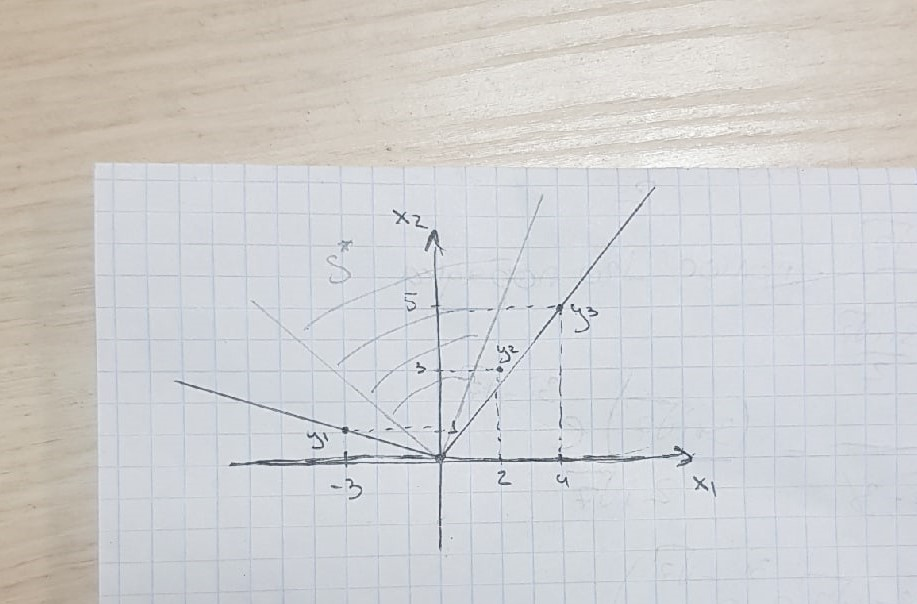
\includegraphics[width=0.7\linewidth]{pic_1}
\label{fuuuu} %% метка рисунка для ссылки на него
\end{center}
\end{minipage}
\end{figure} 

Теперь использую теорему, доказанную на семинаре, что сопряжённым к множеству 
$$
S=\operatorname{conv}\left(x_{1}, \ldots, x_{k}\right)+\operatorname{cone}\left(x_{k+1}, \ldots, x_{m}\right)
$$
является многогранник
$$
S^{*}=\left\{p \in \mathbb{R}^{n} \mid\left\langle p, x_{i}\right\rangle \geq-1, i=\overline{1, k} ;\left\langle p, x_{i}\right\rangle \geq 0, i=\overline{k+1, m}\right\}
$$

В нашем случае: $ S = \mathbf{cone} \{ y_1, y_3\} $, следовательно, $$ S^* = \{ p=\left(\begin{array}{l}
p^{1} \\
p^{2}
\end{array}\right) \in R^n | \quad p^T y_1 \geq 0; \quad p^T y_3 \geq 0 \}
$$
То есть $ S^* $ задаётся как: 
$$
\begin{array}{l}
p^{1} \cdot(-3)+p^{2} \cdot 1  \geqslant 0 \\
p^{1} \cdot (4)+p^{2} \cdot 5 \geqslant 0
\end{array}
$$
Изображено на том же рисунке.


\subsection*{Задача 5}
Find and sketch on the plane a conjugate set to a multifaced cone: 
    
$$
S = \mathbf{conv} \left\{ (-4,-1), (-2,-1), (-2,1)\right\} + \mathbf{cone} \left\{ (1,0), (2,1)\right\} 
$$

Изобразим наше множество: передвигаем конус (коническая оболочка $ y_4, y_5 $) по треугольнику, который получается как выпуклая оболочка точек $ y_1, y_2, y_3 $. В итоге он заметает область, закрашенную на рисунке 

\begin{figure}[h!]
\begin{minipage}[h]{1\linewidth}
\begin{center}
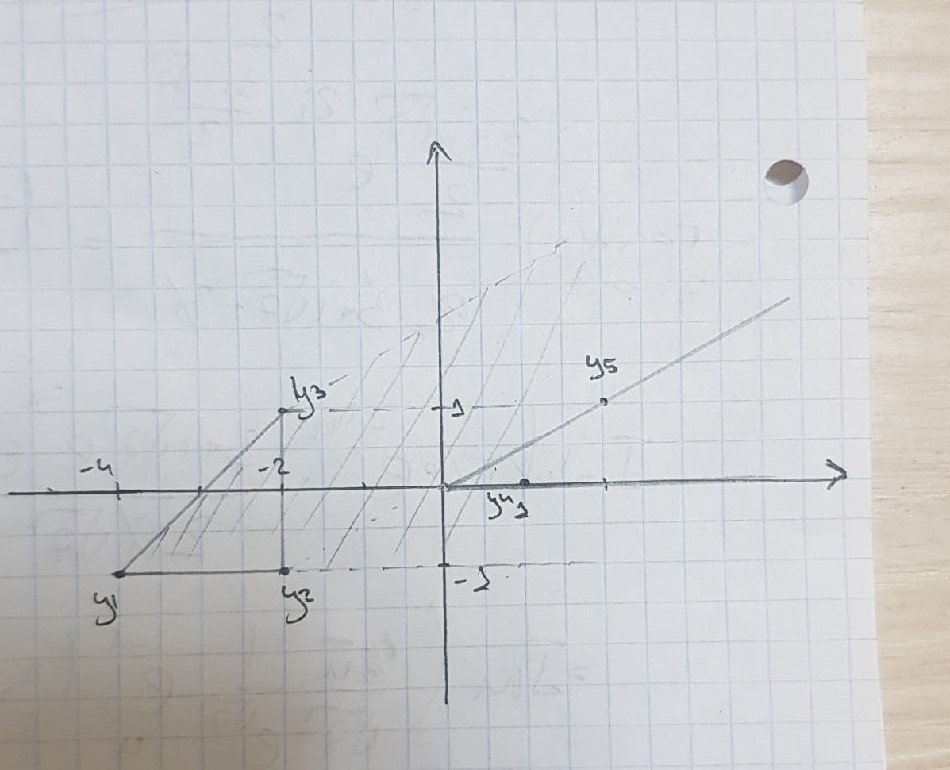
\includegraphics[width=0.7\linewidth]{pic_2}
\label{fuuuu} %% метка рисунка для ссылки на него
\end{center}
\end{minipage}
\end{figure} 

Используем ту же теорему, что и в предыдущей задаче, получаем неравенства:

$$
\left\{\begin{array}{l}
-4 p^{1}-1 p^{2} \geq-1 \\
-2 p^{1}-1 p^{2} \geq-1 \\
-2 p^{1}+p^{2} \geq-1 \\
p^{1} \geq 0 \\
2 p^{1}+p^{2} \geq 0
\end{array}\right.
$$

Построим полученное множество: 
\begin{figure}[h!]
\begin{minipage}[h]{1\linewidth}
\begin{center}
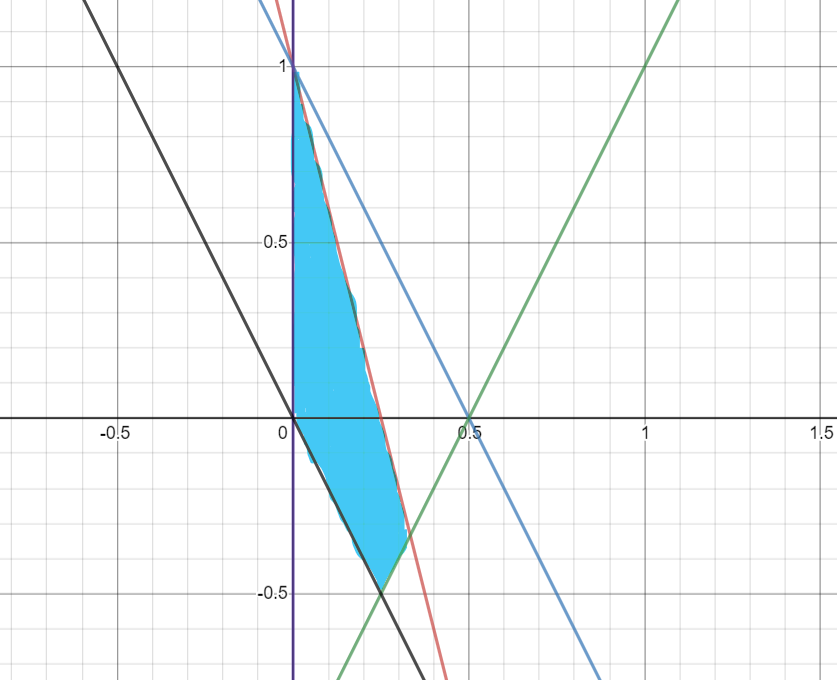
\includegraphics[width=0.7\linewidth]{p5_2}
\label{fuuuu} %% метка рисунка для ссылки на него
\end{center}
\end{minipage}
\end{figure} 

\newpage

\subsection*{Задача 2}
Find the sets $S^{*}, S^{**}, S^{***}$, if     
$$
S = \{ x \in \mathbb{R}^2 \mid x_1 + x_2 \ge 0, \;\; 2x_1 + x_2 \ge -4, \;\; -2x_1 + x_2 \ge -4\}
$$

Изобразим наше множество $ S $:
\begin{figure}[h!]
\begin{minipage}[h]{1\linewidth}
\begin{center}
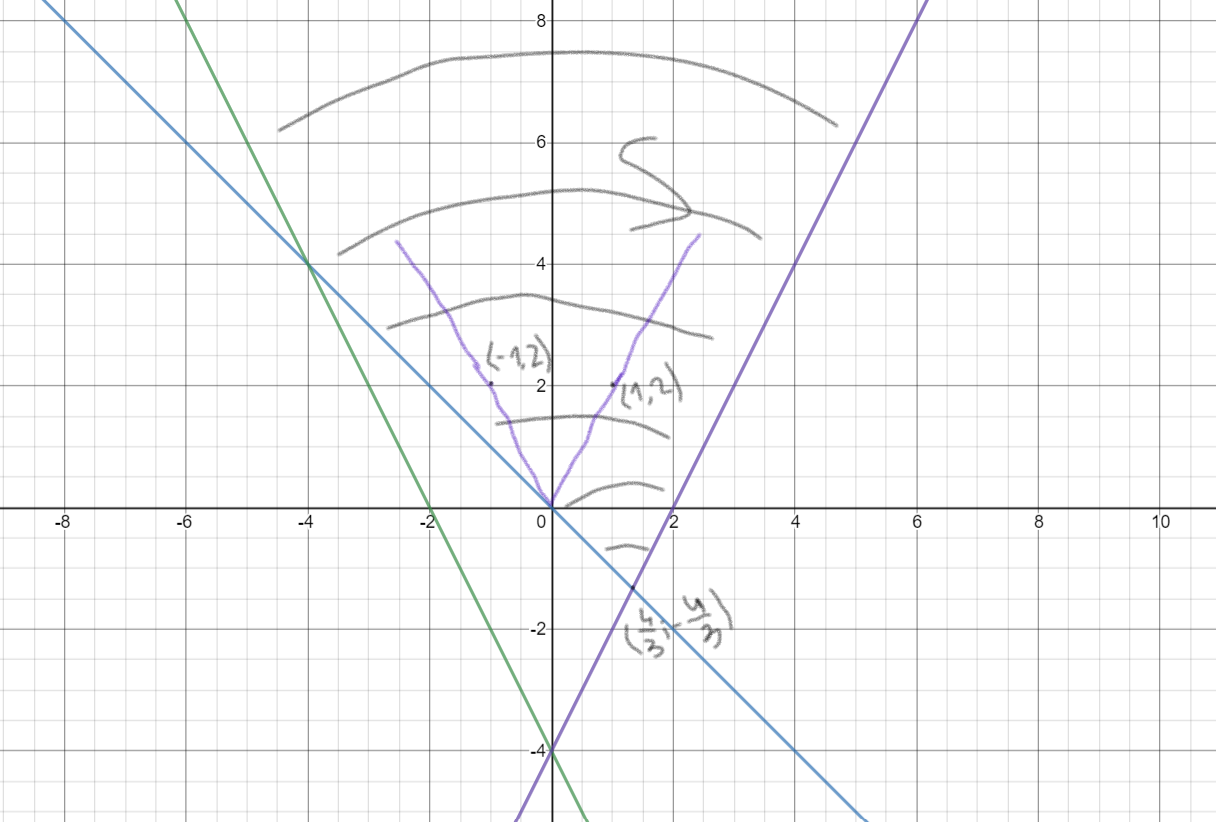
\includegraphics[width=0.7\linewidth]{p2_11}
\label{fuuuu} %% метка рисунка для ссылки на него
\end{center}
\end{minipage}
\end{figure}

Видим, что его можно задать, как 
$$
S=\operatorname{conv}\left((-4, 4), (\frac{4}{3}, -\frac{4}{3}) \right)+\operatorname{cone}\left((1,2), (-1, 2) \right)
$$

Используем теорему, получаем следующие неравенства: 

$$
\left\{\begin{array}{c}
-4 p^{1}+4 p^{2} \geq-1 \\
4 p^{1}-4 p^{2} \geq-3 \\
p^{1}+2 p^{2} \geq 0 \\
-p^{1}+2 p^{2} \geq 0
\end{array}\right.
$$

Изобразим $ S^* $:
\begin{figure}[h!]
\begin{minipage}[h]{1\linewidth}
\begin{center}
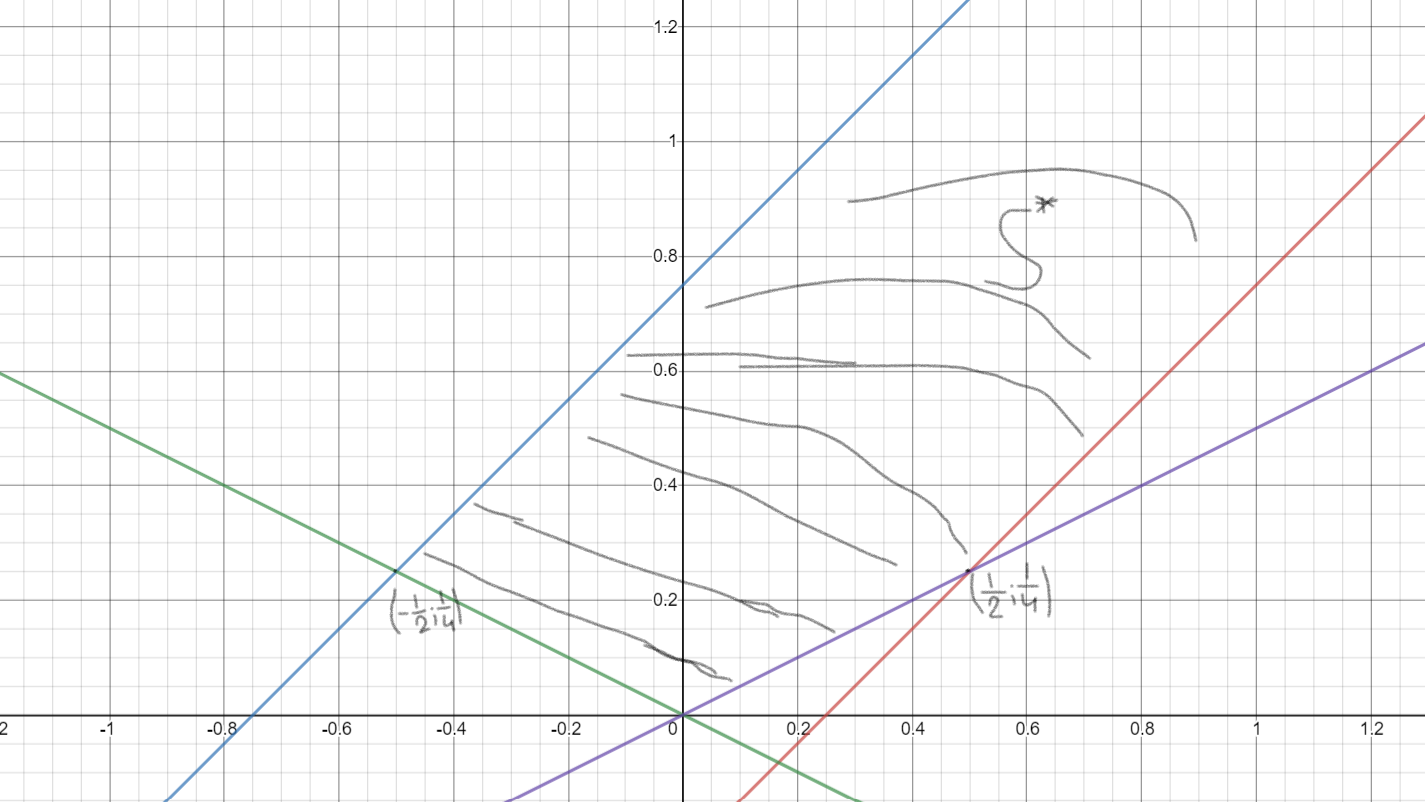
\includegraphics[width=0.7\linewidth]{p2_2}
\label{fuuuu} %% метка рисунка для ссылки на него
\end{center}
\end{minipage}
\end{figure}

Видим, что множество $ S^* $ можно задать как: 
$$
S^*=\operatorname{conv}\left(\left(-\frac{1}{2}, \frac{1}{4} \right), \left( 0,0 \right),  \left( \frac{1}{2}, \frac{1}{4} \right) \right)+\operatorname{cone}\left((1,1) \right)
$$
Прямой $ p^2 = p^1 $ бегаем по треугольнику (который получается как выпуклое множество 3х точек) и заметам как раз нужную нам область.\\
Снова можем приметить теорему и получить такие ограничения на множество $ S^{**} $:
$$
\left\{\begin{array}{l}
-2 p^{1}+p^{2} \geq-4 \\
2 p^{1}+p^{2} \geq-4 \\
p^{1}+p^{2} \geq 0
\end{array}\right.
$$

Построим его:
\begin{figure}[h!]
\begin{minipage}[h]{1\linewidth}
\begin{center}
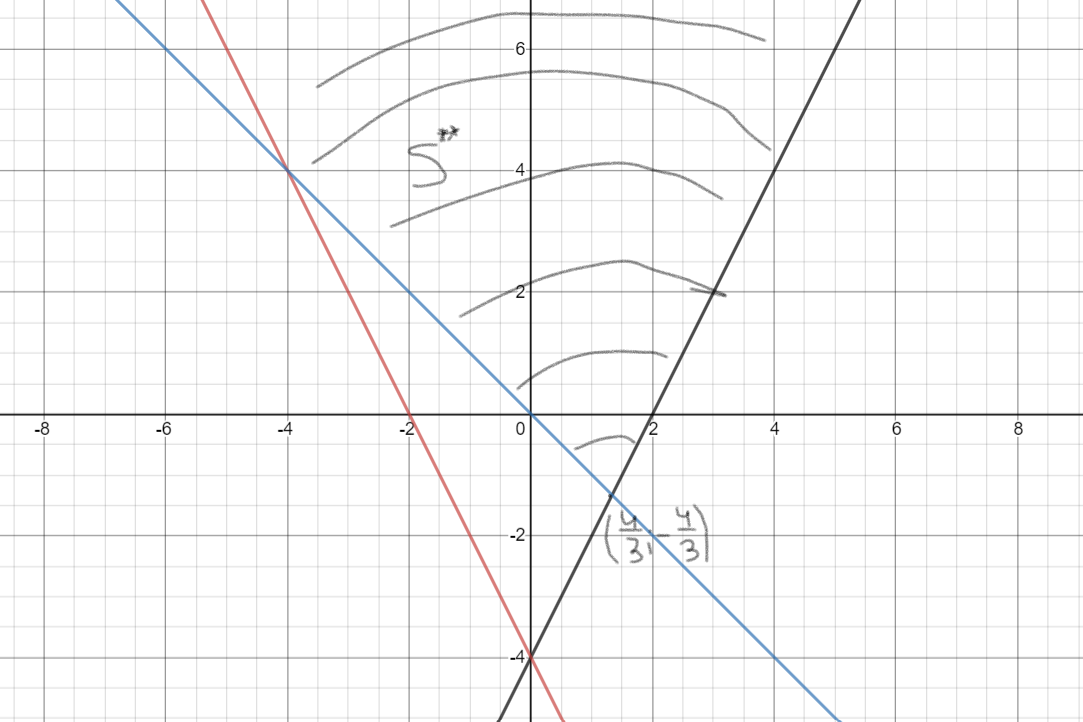
\includegraphics[width=0.7\linewidth]{p2_3}
\end{center}
\end{minipage}
\end{figure}

\newpage

Видим, что $ S = S^{**} $! (все ограничения на множества совпадают). Также на семинаре было свойство, что если $ S $ - замкнуто (в нашем случае это так, так как все неравенства нестрогие), выпукло и включает 0, то $ S^{**} = S $, что и получили.\\  Следовательно, $ S^{***} = S^{*} $, которое уже нашли выше. 



\subsection*{Задача 3}
Let $\mathbb{A}_n$ be the set of all $n$ dimensional antisymmetric matrices. Show that $\left( \mathbb{A}_n\right)^* = \mathbb{S}_n$. \\

Покажем вложения в обе стороны. Сначала, что $ \left( \mathbb{A}_n\right)^* \subset \mathbb{S}_n  $.\\
пусть матрица $ B \in \left( \mathbb{A}_n\right)^* $ . $ \forall A $ - антисимметричной (то есть $ A^T = -A $) 
$$ tr \left( A^T B \right) = tr \left( A B^T \right) \geq -1  $$
Пользуясь тем, что $ A^T = -A $, получаем:
$$ tr \left( -AB \right) \geq -1 $$
$$ tr \left( A B^T \right) \geq -1$$
Складываем эти 2 неравенства, получаем:
$$ tr \left( A \cdot (B^T-B) \right) \geq -2 $$
$$
tr \left( A \cdot (B- B^T) \right) \leq 2
$$
Мы хотим показать, что матрица $ B \in  \mathbb{S}_n $, то есть, что $ B = B^T $. Докажем это от противного, пусть $ B \neq B^T $ тогда у матрицы $ B-B^T $ на диагонале стоят 0 (так как эти элементы не меняются при транспонировании) и есть хотя бы один ненулевой элемент. Матрица $ A $ - произвольная антисимметричная (значит на диагонали у неё тоже стоят нули). Так как матрица $ A $ произвольная, то выберем её элементы таким образом, чтобы на диагонали у матрицы $ A (B-B^T) $ был хотя бы 1 элемент.\\ Мы так можем сделать всегда, так как: пусть без ограничения общности ненулевой элемент у матрицы $ (B-B^T) $ будет в первом столбце: $ b_{i1} $ (но не на диагонале). Тогда в первой строке матрицы $A$ выбираем $ a_{1i} \neq 0 $ а остальные равные нулю. Следовательно при произведении получаем, на диагонале ненулевой элемент: $ e = b_{i1} \cdot a_{1i}  $.\\
След матрицы равен сумме диагональных  элементов. Б.о.о. пусть у $ (B-B^T) $ только 1 ненулевой элемент, значит  $ tr \left( A \cdot (B- B^T) \right) = e $. Так как матрица $ A $ произвольная, то можем взять её с элементом  $a_{1i} \cdot \frac{10}{e} $. Тогда $ tr \left( A \cdot (B- B^T) \right) = 10 > 2 $ получаем противоречие, что $ B \in \left( \mathbb{A}_n\right)^* $.\\ Это случай, когда в матрице $ (B-B^T) $ 1 ненулевой элемент, но это вообще не обязательно так, может быть 2 и в итоге мы не покажем этими рассуждениями, что след равен 0. Рассмотрим более стого: \\
заметим, что матрица $ (B-B^T) $ - антисимметричная (простой факт из линейной алгебры), поэтому нам нужно показать, что для произвольной антисимметричной матрицы $ B^* =  (B-B^T) $ можно подобрать такую антисимметричную $ A $, что $ tr (A B^*) \neq 0$, это так, так как если мы просто будем брать такую же, то будем получать отрицательно определённую (на диагонале будут стоять числа одного знака и след не занулится), ну а дальше аналогично рассуждениям выше можем взять $ A $ такую, что след произведения был больше двух и мы получим противоречие 

 


Значит, $ B = B^T $, то есть симметричная: $ B \in \mathbb{S}_n \rightarrow \left( \mathbb{A}_n\right)^* \subset \mathbb{S}_n $\\

Покажем вложение в другую сторону: пусть $ B \in \mathbb{S}_n $, то есть $ B = B^T $ а $ A $ - произвольная антисимметричная матрица, тогда: 
$$
tr (A B^T) = tr(AB) 
$$
$$
tr(A^T B) = - tr (AB)
$$
Получается, что $ tr(AB)=-tr(AB) \rightarrow tr(AB) = 0 > -1 $, значит $ B \in \left( \mathbb{A}_n\right)^* \rightarrow \left( \mathbb{A}_n\right)^* \supseteq \mathbb{S}_n$\\

Показав вложения друг в друга получаем, что $\left( \mathbb{A}_n\right)^* = \mathbb{S}_n$


\subsection*{Задача 4}
Find the conjugate cone for the exponential cone:
$$
K = \{(x, y, z) \mid y > 0, y e^{x/y} \leq z\}
$$

Рассуждаем по определению: нам нужно найти такие вектора из $ R^3 $ с коэффициентами $ (a, b, c) $ такие что: 
$$
(x, y, z)\left(\begin{array}{l}
a \\
b \\
c
\end{array}\right) \geq 0, \; \text{где}(x, y, z):\left\{\begin{array}{l}
y e^{x / y} \leq z \\
y>0
\end{array}\right.
$$

Сделаем замену: обозначим за $ u = \frac{x}{y} $ и $ v = \frac{z}{y} $, тогда получим условие:
$$a u+b+c v \geq 0, \quad \text{где} \; (u, v): \left\{\begin{array}{l}
v>0 \\
v \geq e^{u}  \; 
\end{array}\right. $$ 
Так как $ K^* $ - конус, то можно рассмотреть только 3 случая: $ c = -1 $, $ c = 0 $, $ c = 1 $ все остальные случаи получаются домножением на положительную константу.\\

Рассмотрим $ c = 1 $. Нам нужно подобрать такие $ a,b $, что в области $ v \geq -au - b $ лежали все значения $v \geq e^{u}$. Решаем это графически: строим множество точек  $v \geq e^{u}$ и смотрим, как может распологаться прямая $v = -au - b$. Попередвигая прямую в desmos получааем:

\begin{figure}[h]
\begin{center}
\begin{minipage}[h]{0.4\linewidth}
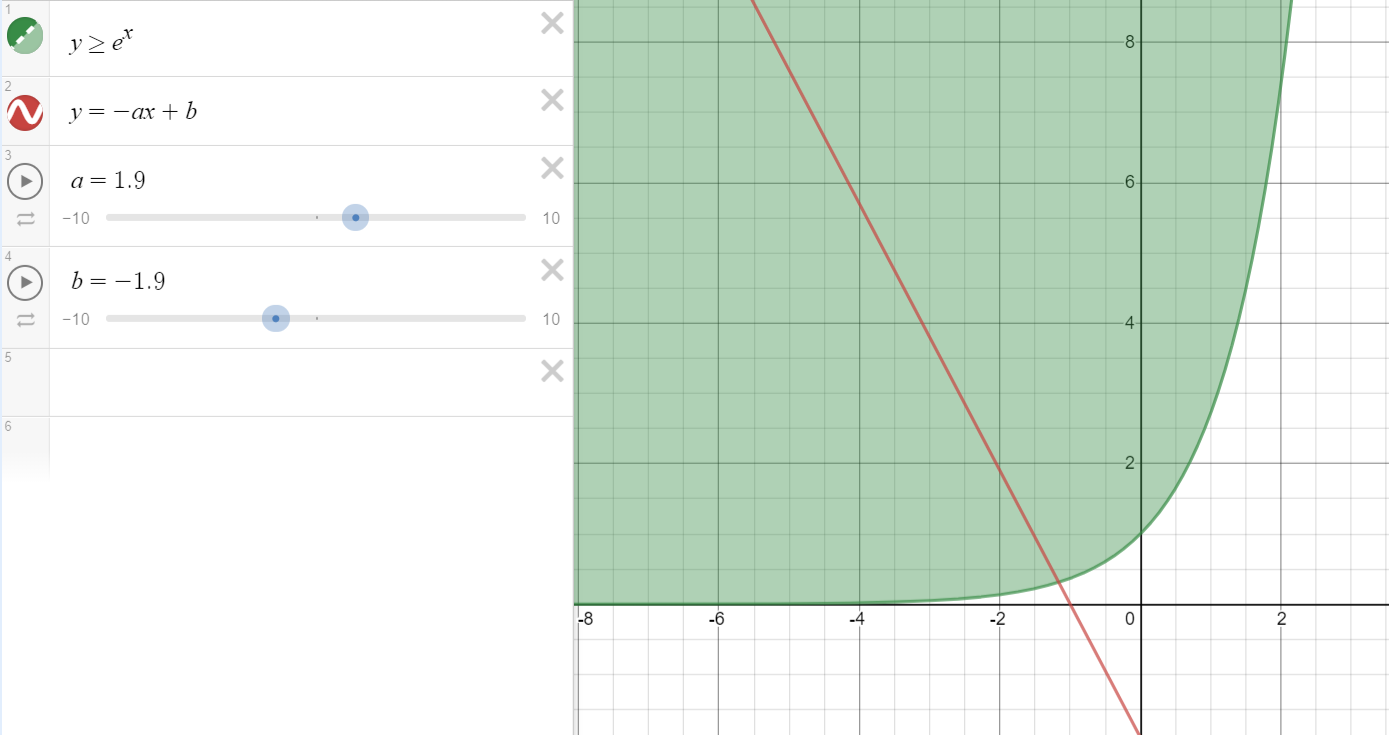
\includegraphics[width=1\linewidth]{graph_sol_1}
\caption{$a > 0$} %% подпись к рисунку
%%\label{ris:experimoriginal} %% метка рисунка для ссылки на него
\end{minipage}
\hfill
\begin{minipage}[h]{0.4\linewidth}
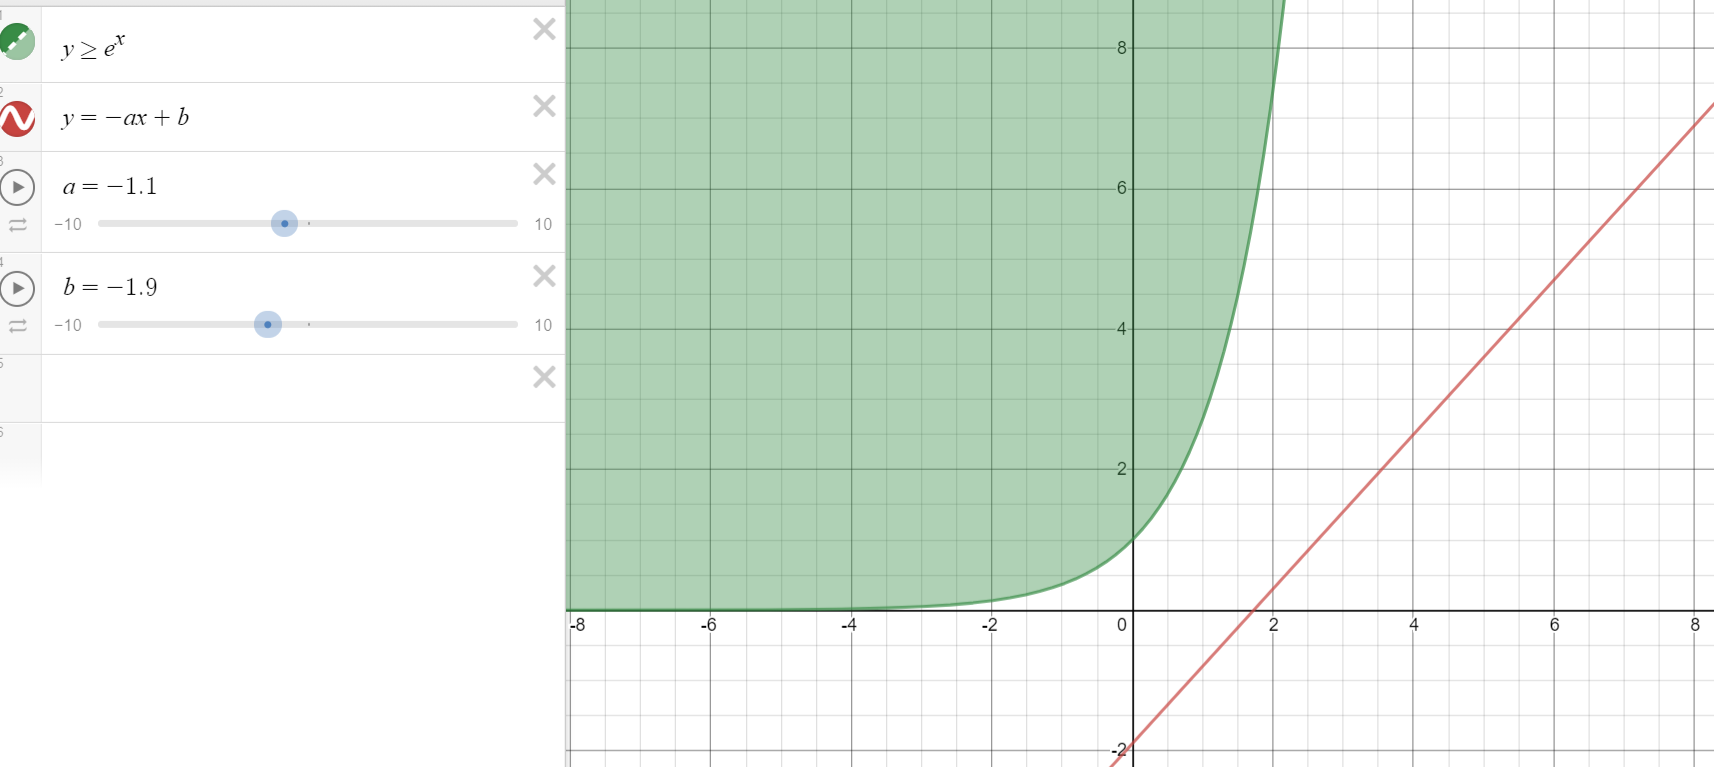
\includegraphics[width=1\linewidth]{graph_sol_2}
\caption{$a<0$}
%%\label{ris:experimcoded}
\end{minipage}
\end{center}
\end{figure}

Делаем такие выводы: при $ a > 0 $ - невозможно (зелёная зона должна быть полностью выше прямой). При $ a = 0 $ это возможно только при $ b \geq 0 $. При $ a < 0 $ ситуация сложнее. Для понимания подходящих условий найдём точку касания кривых: $v \geq e^{u}$ и $v = -au - b$ для этого приравниваем значения функции и её производной, получаем связь коэффициентов $ b $ и $ a $:

$$
\left\{\begin{array}{l}
e^{u}=-a u-b \\
e^{u}=-a
\end{array} \quad \Longrightarrow \quad b=a(1-\ln (-a))\right.
$$

В итоге для случая $ c=1 $ получаем: 
$$
\begin{aligned}
&\begin{array}{l}
a<0: \quad b \geq a(1-\ln (-a)) \\
a=0: \quad b \geq 0
\end{array}\\
&a>0: \text { нет подходящих } b
\end{aligned}
$$

Теперь рассмотрим $ c = 0 $ то есть в области $ au+b \geq 0 $ лежат все точки $v \geq e^{u}$, но таких $ a $ и $ b $ мы не найдём, так как $ au+b = 0 $ - вертикальная прямая поэтому понятно, что не при каких $ a $ и $ b $ не получим нужное нам условие.\\

Для случая $ c < 0 $ множество точек  $v \geq e^{u}$ должно лежать выше прямой $ au+b \geq v $, что не выполняется не при каких $ a $ и $ b $ (можно также понять графически). Если строго, то множество $v \geq e^{u}$ не ограничено сверху, а прямая делает это ограничение, следовательно, не при каких $ a $ и $ b $ наши требования не выполнятся.\\

Разобрав все случаи можем записать ответ: помним, что так как мы ищем сопряжённый конус, то все полученные тройки можно домнажать на произвольную положительную константу - $ \alpha $, и заметим, что если все три коэффициента будут равняться 0, то такой вектор тоже принадлежит нашему сопряжённому конусу (по определению), поэтому:
$$
K^{*}=\left\{ \alpha \cdot (a, b, 1) \mid \alpha \geq 0, \begin{array}{l}
\text { при } a=0, \text { и } b \geq 0 \\
\text { при } a<0, \text { и } b \geq a(1-\ln (-a))
\end{array}\right\}
$$



 
\subsection*{Задача 6}
Prove that if we define the conjugate set to $S$ as follows:  
$$
S^* = \{y \ \in \mathbb{R}^n \mid \langle y, x\rangle \le 1 \;\; \forall x \in S\}, 
$$
then unit ball with the zero point as the center is the only self conjugate set in $\mathbb{R}^n$.\\

Для такого определения хотим найти множество $ S $, такое что $ S = S^* $ (то есть самосопряжённое). Зафиксируем какой-то элемент $ p \in S^* $: по определению: $ \forall x \in S \rightarrow  \langle y, x\rangle \le 1$, то есть $ \max\limits_{x \in S} \; x^T p \le 1 $.\\
Заметим, что если $ |p| >1 $, то мы можем взять $ x = p $ (так как $ S = S^* $) но $ p^2 > 1 $, следовательно $ p \notin S^* $. Получили противоречие, значит $ |p| \le 1 $ (показали, что если во множестве есть хотя бы один элемент норма которого больше 1, то такое множество уже не может быть самосопряжённым по введённому определению).\\

Покажем, что единичный шар с центром в нуле будет самосопряжён: действительно геометрически (и из свойств скалярного произведения) понятно, что чтобы максимизировать $ \max\limits_{x \in S} \; x^T p $ для фиксированного $ p $ из единичного шара нужно брать $ x = \frac{p}{\| p \|} \| x \| $. Значит, $ p \le \frac{1}{\| x \|}  \rightarrow p \le 1$ (так как $ x $ - произвольный из $ S $).\\ Обратное включение: $ \forall p \in S^* = B_{r = 1} $ и $ \forall x \in S = B_{r = 1} $ $ \quad x^T \cdot p \le 1 $ (следует из неравенства Коши-Буняковского и того, что оба элемента из единичного шара), следовательно, верно обратное включение и значит $ S = S^* = B_{r = 1} $  \\

Покажем, что шары с меньшим радиусом, не будут самосопряжёнными. Рассмотрим шар радиусом $ r < 1 $, тогда сопряжённым к нему будет шар радиусом $ \frac{1}{r} $. \\
Так как для фиксированного $ p \in S^* \in B_{\frac{1}{r}} $  $ \max\limits_{x \in S} \; x^T p $ достигается при $ x \in S $ сонаправленном с $ p $, то из определения сопряжённого множества: $ x^T \cdot p \le 1 \rightarrow p \le \frac{1}{r} $, тем самым показали включение $ B_{\frac{1}{r}} \subseteq S^* $\\
Обратное включение:
$ x^T p \le \frac{1}{r} \cdot r = 1 \le 1 $, следовательно, $ S^* \subseteq  B_{\frac{1}{r}} $. \\
Но для $ r < 1 $, $ B_r \neq B_{\frac{1}{r}} $, значит, не является самосопряжённым. \\

Покажем, что множество произвольной формы, которое лежит в шаре радиусом 1 не будет являться самосопряжённым (можно было не доказывать абзац выше, но не дошла такая идея сразу): \\
рассмотрим произвольное $ S \subset B_{r=1} $, по определению сопряжённого множества для $ p \in S^* $, $ \forall x \in S \rightarrow x^T p \leq 1 $.\\
Рассматриваем $ S = S^* \neq B_{r=1} $, следовательно, $ \exists z \notin S $ и $ z \in B_{r=1} $.\\ Так как $ z $ лежит в единичном шаре, то $ \| z \| \leq 1 $, следовательно:\\
$ \forall x \in S \subset B_{r=1} \rightarrow z^T x \leq 1 $, значит по определению $ z \in S = S^* $.\\ Получаем противоречие, что $ z $ принадлежит и не принадлежит $ S $, значит множества произвольной формы лежащие внутри единичного шара не могут быть самосопряжёнными.


Показали, что множества произвольной формы, где есть элемент с модулем больше 1, не могуть быть самомсопряжёнными. Что единичный шар - самосопряжённое множество и что все множества, которые вложены в него не будут самосопряжёнными.

Значит, для такого определения только единичный шар с центром в точке 0 является самомсопряжённым.

\subsection*{Задача 7}
Find the conjugate set to the ellipsoid: 
$$
S = \left\{ x \in \mathbb{R}^n \mid \sum\limits_{i = 1}^n a_i^2 x_i^2 \le \varepsilon^2 \right\}
$$

Перепишем определение конуса через матрицу, чтобы было удобнее работать: 

$$
S = \left\{ x \in \mathbb{R}^n \mid \sum\limits_{i = 1}^n \left( \frac{a_i}{\varepsilon} \right) ^2  x_i^2 \le 1 \right\}
$$

Рассмотрим матрицу $ A = \operatorname{diag} (\frac{a_i}{\varepsilon}) $ - диагональная матрица, тогда $$ \| Ax \|_2^2 = 
 \sum\limits_{i = 1}^n \left( \frac{a_i}{\varepsilon} \right) ^2  x_i^2 $$
 
Поэтому задать эллипс мы можем как:
$$
S = \left\{ x \in \mathbb{R}^n \mid \| Ax \|_2  \le 1 \right\}
$$

покажем, что такое задание эллипса эквивалентно следующему (откуда придумал такой вид? - в Бойде в теме convex set, нашёл, что можно задавать так и это сильно помогло упростить решение):

$$
E = \left\{ A^{-1}u \mid \| u \|_2  \le 1 \right\}
$$

Покажем вложение множеств друг в друга, чтобы показать их эквивалентность. \\
Из 2го в 1ое: пусть $ x = A^{-1}u $, где $ \| u \|_2  \le 1 $, подставим в 1ое определение, получим, что $  \|  A A^{-1}u \|_2  \le 1 $ - верно, следовательно, $ E \subseteq S $\\
Из 1го во 2ое: возьмём $ x $ такой что $ \| Ax \|_2  \le 1 $, обозначим $ y = Ax $, получается, что $ \| y \|_2  \le 1 $. Из введённого обозначения выразим $ x: \; x = A^{-1}y $, где $ \| y \|_2  \le 1 $, следовательно $ x \in E $ и $ S \subseteq E $\\
Получаем, что $ E=S $ - один и тот же эллипсойд.

Работаем с определением конуса $ E = \left\{ A^{-1}u \mid \| u \|_2  \le 1 \right\} $, тогда по определению хотим найти все такие векторы $ p \in E^* $, что $ \forall x \in E \rightarrow \langle p, x \rangle \geq -1$, так как любой вектор $ x \in E $ представим как $ x = A^{-1}u $, где $ \| u \|_2  \le 1 $, то нам подходят $ p $ такие что выполнено:
$$
\langle p, A^{-1} u \rangle \geq -1, \; \text{где } \| u \|_2  \le 1
$$
$$
\langle A^{-T} p,  u \rangle \geq -1, \; \text{где } \| u \|_2  \le 1
$$

Применяем неравенство Коши-Буняковского, получаем:
$$
| \langle A^{-T} p,  u \rangle | \leq \| u \|_2 \cdot \| A^{-T} p \|_2 \leq \left[ \| u \|_2 \leq 1 \right] \leq \| A^{-T} p \|_2
$$

Так как вектор $ u $ - произвольный, то равенство может достигаться всегда, поэтому нам подходят все $ p $, для которых выполнено:
$$
-1 \leq - \| A^{-T} p \|_2 \Leftrightarrow \| A^{-T} p \|_2 \leq 1
$$

Такой вид неравенства уже видели выше, оно задаёт эллипс, но теперь с другой матрицей. Заметим, что $ A $ - диагональная, поэтому при транспонировании ничего не меняется, а при взятии обратной все элементы на диагонали становятся обратными (по определению обратной матрицы, чтобы при перемножении с исходной получить единичную), то есть $ A^{-T} = \operatorname{diag} (\frac{\varepsilon}{a_i})$, если переходить к привычному заданию в виде суммы, то получим:

$$
E^* = \left\{ x \in \mathbb{R}^n \mid \sum\limits_{i = 1}^n \left( \frac{\varepsilon}{a_i} \right) ^2  x_i^2 \le 1 \right\}
$$
что эквивалентно
$$
E^* = \left\{ x \in \mathbb{R}^n \mid \sum\limits_{i = 1}^n \left( \frac{1}{a_i} \right) ^2  x_i^2 \le \left( \frac{1}{\varepsilon} \right)^2 \right\}
$$

Чтобы проверить себя можно рассмотреть частный случай эллипсоида - шар (то есть все $ a_i = 1 $), тогда получим сопряжённое множество - шар с радиусом $ \frac{1}{R} $, что верно (рассматривали на семинаре)




\newpage

\section*{Сonjugate function}
\subsection*{Задача 1}
Find $f^*(y)$, if $f(x) = -\dfrac{1}{x}, \;\; x\in \mathbb{R}_{++}$\\

Запишем определение сопряжённой функции: 
$$
f^*(y) = \sup_x \left( xy - f(x) \right) = \sup_x \left( xy + \frac{1}{x} \right) = \sup_x f(x,y)
$$

Посмотрим, на область определения $ f^*(y) $, то есть при каких $ y $, $ \sup\limits_x \left( xy + \frac{1}{x} \right) $ - ограничен. Рассмотрим случаи:
\begin{itemize}
\item[1) ] если $ y > 0 $, то при $ x \rightarrow +\infty $, $ xy \rightarrow +\infty$, а $ \frac{1}{x} \rightarrow 0 $, следовательно $ f(x,y) \rightarrow +\infty $
\item[2) ] если $ y < 0 $, то при $ x \rightarrow -\infty $, $ xy \rightarrow +\infty$, а $ \frac{1}{x} \rightarrow 0 $, следовательно $ f(x,y) \rightarrow +\infty $
\item[3) ] если $ y = 0 $, то $ \forall x \; xy =0   $. При $ x \rightarrow 0 $, то $ \frac{1}{x} \rightarrow + \infty $, следовательно, $ f(x,y) \rightarrow +\infty $
\end{itemize}
Ответ: $ f^*(y) = +\infty $ (или можно сказать, что функция не определена)



\subsection*{Задача 2}
Find $f^*(y)$, if $f(x) = -0,5 - \log x, \;\; x>0 $\\

Запишем определение сопряжённой функции: 
$$
f^*(y) = \sup_x \left( xy - f(x) \right) = \sup_x \left( xy + 0,5 + \log x \right) = \sup_x f(x,y)
$$
Ищем максимум $ f(x,y) $ для этого 
$$ \nabla_{x} f(x,y) = y + \frac{1}{x} = 0 \Rightarrow x^* = -\frac{1}{y}$$
Видим, что область определения $ f^*(y)$: $ y < 0 $ (чтобы $ x\in \mathbb{R}_{++} $), по определению:
$$
f^*(y) =  f(x^*,y) = y \cdot \left( -\frac{1}{y} \right) + \log \left( -\frac{1}{y} \right) + 0,5 = -0,5 - \log (-y)
$$
Ответ: $ f^*(y) = -0,5 - \log (-y) $, область определения $ y < 0 $ то есть:

$$
f^{*}(y)=\left\{\begin{array}{ll}
-0,5 - \log (-y) & \text {,  при } y<0 \\
+\infty & \text { , при } y \geq 0
\end{array}\right.
$$



\subsection*{Задача 3}
Find $f^* (y)$, if $ f(x) = \log \left( \sum\limits_{i=1}^n e^{x_i} \right) $ \\

По определению сопряжённой функции: 
$$
f^{*}(y)=\sup _{x \in \operatorname{dom} f}(\langle y, x\rangle-f(x))
$$
Взяв градиент по $ x $ от функции $ \langle y, x\rangle-f(x) $ и приравняв его к нулю (для нахождения максимума (супремума)), получаем такие равенства: 
$$
y_{i}=\frac{e^{x_{i}}}{\sum_{j=1}^{n} e^{x_{j}}}, \quad i=1, \ldots, n
$$
Если подставить в определение для двойственной функции, получим:
$$
f^*(y) = \sum\limits_{i=1}^n y_i x_i - \log \left( \sum\limits_{i=1}^n e^{x_i} \right) = \sum\limits_{i=1}^n \log e^{x_i y_i} - \log \left( \sum\limits_{i=1}^n e^{x_i} \right) = \sum\limits_{i=1}^n
 \log  \frac {e^{x_i} e^{y_i} }{ \sum\limits_{i=1}^n e^{x_i} } = \sum\limits_{i=1}^n y_i \log y_i
$$

Получили, что $ f^*(y_i) = y_i \log y_i $ - знакомая нам кросс-энтропия!, ведь это верно, тогда и только тогда когда $
y \succ 0 \text { and } \mathbf{1}^{T} y=1
$ (что соответствует, что $ y $ - вектор вероятности: все $ y_i > 0 $ и $ \sum \limits_{i = 1}^n y_i = 1 $  ). \\
Покажем, что область определения $ f^*(y) $ это как раз вектора вероятности: 
\begin{itemize}
\item пусть существует компонента вектора $ y $, такая что $ y_i < 0 $, тогда возьмём вектор $ x $ таким: $
x_{k}=-t, \text { и } x_{i}=0, i \neq k
$ и устремим $ t $ к бесконечности. Получаем, что $ y^{T} x-f(x) $ стремится к бесконечности, как $ t - \log t $, следовательно $ f^*(y) $ - неограничена. 
\item $ \text { Если } y \succeq 0 \text { но } \mathbf{1}^{T} y \neq 1, \text { выберем } x=t \mathbf{1}, \text { получим } $
$$
y^{T} x-f(x)=t \mathbf{1}^{T} y-t-\log n
$$
Если $ \mathbf{1}^{T} y > 1 $, то  $ f^*(y) $ - неограничена при $ t \rightarrow \infty $\\
если $ \mathbf{1}^{T} y < 1 $, то  $ f^*(y) $ - неограничена при $ t \rightarrow -\infty $
\end{itemize}
В итоге: 
$$
f^{*}(y)=\left\{\begin{array}{ll}
\sum_{i=1}^{n} y_{i} \log y_{i} & \text { если } y \succeq 0 \text { и } \mathbf{1}^{T} y=1 \\
\infty & \text { иначе }
\end{array}\right.
$$
то есть сопряжённая функция - кросс-энтропия для $ y $ - вектора вероятности.


\subsection*{Задача 4}
Prove, that if $f(x) = \alpha g(x)$, then $f^*(y) = \alpha g^*(y/\alpha)$\\

По определению сопряжённой функции: 
$$
\begin{aligned}
f^{*}(y) &=\sup _{x} (x y-f(x))=\sup _{x}(x y-\alpha g(x))=\\
&=\sup _{x} \left(\alpha\left[x \cdot \frac{y}{\alpha}-g(x)\right]\right)=\left[ \alpha>0\right]=\alpha \sup _{x} \left(x \cdot \frac{y}{\alpha}-g(x)\right) =\\
&= \alpha \cdot g^* \left( \frac{y}{\alpha} \right)
\end{aligned}
$$
Получили то, что нужно: $f^*(y) = \alpha g^*(y/\alpha)$

\subsection*{Задача 5}
Find $f^*(Y)$, if $f(X) = - \ln \det X, X \in \mathbb{S}^n_{++}$
По определению сопряжённая функция определяется как: 
$$
f^{*}(Y)=\sup _{X \succ 0}(\operatorname{tr}(Y^T X)+\log \operatorname{det} X)
$$
используем $ \operatorname{tr}(Y^T X) $ как операцию скалярного умножения на матрицах. Заметим, что $ f^{*}(Y) $ неограничена, если $ Y \nprec 0 $, так как тогда $ Y $ имеет собственный вектор $ v $ с $ \lambda \geq  0 $ и без ограничения общности $ \|v\|_{2}=1 $, тогда возьмём $ X=I+t v v^{T} $, получим: 
$$
\operatorname{tr}(Y^T X)+\log \operatorname{det} X=\operatorname{tr} Y^T+t \lambda+\log \operatorname{det}\left(I+t v v^{T}\right)=\operatorname{tr} Y^T+t \lambda+\log (1+t)
$$
Видим, что неограничено при $ t \rightarrow \infty $.\\
Если $ Y \prec 0 $, то найдём максимум, взяв градиент по матрице $ X $ (из первого задания знаю, что $ \nabla_{X} \log \operatorname{det} X = X^{-1}$ и $ \nabla_{X} \operatorname{tr}(Y^T X) = Y $), получаем:
$$
\nabla_{X}(\operatorname{tr}(Y^T X)+\log \operatorname{det} X)=Y+X^{-1}=0
$$
что даёт: $ X = -Y^{-1} $ (видим, что $ X $ - положительно определена, значит подходит. Ещё так как $ X $ - симметричная, то $ Y $ тоже должна быть симметричной), подставляя в определение, получаем \\
Ответ:
$$
f^{*}(Y)=\log \operatorname{det}(-Y)^{-1}-n
$$
область определения: $ \operatorname{dom} f^{*}=-\mathbf{S}_{++}^{n} $

\subsection*{Задача 6}
Prove, that if $f(x) = g(Ax)$, then $f^*(y) = g^*(A^{-\top}y)$\\
Доказываем по определению функции $ f^{*}(y) $, затем сводим к определению функции $ g^* $ 
$$
f^{*}(y)=\sup _{x}\left(x^{\top} y-f(x)\right)=\sup _{x} p\left(x^{\top} y-g(A x)\right)=
$$
$$
=\left[z=A x, \quad x=A^{-1} z\right]=\sup _{z} \left( \left( A^{-1} z \right)^{\top} y-g(z)\right)=
$$
$$
=\sup _{z} \left(z^{\top} A^{-T} y-g(z)\right)=g^{*}\left(A^{-T} y\right)
$$
Можем переходить от супремума по $ x $ к супремуму по $ z $, так как $ z=A x $ - линейная замена.\\
Получили, что $f^*(y) = g^*(A^{-\top}y)$

\newpage
\section*{Subgradient and subdifferential}
\subsection*{Задача 1}
Prove, that $x_0$ - is the minimum point of a convex function $f(x)$ if and only if $0 \in \partial f(x_0)$\\

По определению $ g $ - субградиент $ f(x) : S\rightarrow R $ в точке $ x_0 $, если $ \forall x \in S $
$$
f(x) \geq f\left(x_{0}\right)+\left\langle g, x-x_{0}\right\rangle
$$
Множество всех субградиентов $ f(x) $ в точке $ x_0 $ - субдифференциал $ f $ в $ x_0 $. 
$$ 0 \in \partial f(x_0) \longrightarrow f(x) \geq f\left(x_{0}\right), \quad \forall x \in S $$
Но это и есть определение минимума выпуклой функции! (так как $ f(x) $ - выпуклая, то $ \forall x \in S $, а не для окрестности $ x_0 $). Получаем, что утверждения эквивалентны. 

\subsection*{Задача 2}
Find $\partial f(x)$, if $f(x) = \text{ReLU}(x) = \max \{0, x\}$\\

По теореме Дубовитского-Милютина, так как $ 0 $ и $ x $ - выпуклые функции на выпуклом множестве $S \subseteq \mathbb{R}^{n} $ 
$$
\begin{array}{r}
\partial_{S} f\left(x_{0}\right)=\operatorname{conv}\left\{\bigcup\limits_{i \in I\left(x_{0}\right)} \partial_{S} f_{i}\left(x_{0}\right)\right\} \\
\text { где } I(x)=\left\{i \in[1: m]: f_{i}(x)=f(x)\right\}
\end{array}
$$

Применяя эту теорему (при $ x > 0 $ - активная функция $ y = x $, при $ x < 0 $ - активная функция $ 0 $, в точке 0 обе функции активны, поэтому берём выпуклую оболочку), получим: 
$$
\partial f(x)=\left\{\begin{array}{l}
1, \quad x>0 \\
\{0\}, \quad x<0 \\
\left\{a \mid a=\lambda a^{\prime}, 0 \leq \lambda \leq 1, a^{\prime} \in \partial x = 1 \right\}, \quad x=0
\end{array}\right.
$$

\subsection*{Задача 3}
Find $\partial f(x)$, if $f(x) = \|x\|_p$ при $p = 1,2, \infty$\\

Сначала напишем для $ f(x) = \| x \|_1 $, по определению это:

$$
\|x\|_{1}=\left|x_{1}\right|+\left|x_{2}\right|+\ldots+\left|x_{n}\right|=s_{1} x_{1}+s_{2} x_{2}+\ldots+s_{n} x_{n}
$$
где $ s_i = \{ -1, 1 \} $\\
Рассмотрим эту функцию, как поточечный максимум линейных по $ x $ функций, по теореме Дубовицкого-Милютина в каждой точке 
$$
\partial f=\operatorname{conv}\left(\bigcup_{i \in I\left(x\right)} \partial g_{i}(x)\right)
$$

где субдифференциал $ g $ в силу её линейности определяется как ($ \partial g_i(x) = \nabla g_i(x) = s_i $):

$$
\partial g(x)=\partial\left(\max \left\{s^{\top} x,-s^{\top} x\right\}\right)=\left\{\begin{array}{ll}
-s, & s^{\top} x<0 \\
\operatorname{conv}(-s ; s), & s^{\top} x=0 \\
s, & s^{\top} x>0
\end{array}\right.
$$

и <<активные>> индексы в каждой точке мы выбираем как (в одномерном случае):
\begin{itemize}
\item  Если j-ая координата точки отрицательна, $s_i^j = -1$
\item Если j-ая координата точки положительна, $s_i^j = 1$
\item Если j-ая координата точки равна нулю, то подходят оба варианта коэффициентов и соответствующих им функций, а значит, необходимо включать субградиенты этих функций в объединение в теореме Дубовицкого - Милютина
\end{itemize}

Чтобы красиво записать ответ, рассмотрим двумерный случай:
\begin{figure}[h!]
\begin{minipage}[h]{1\linewidth}
\begin{center}
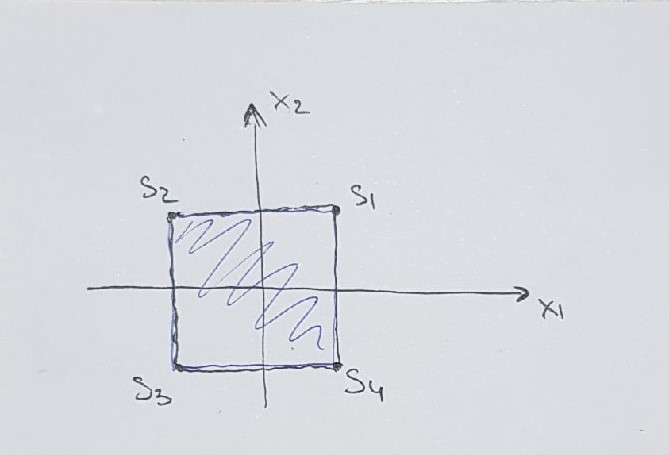
\includegraphics[width=0.7\linewidth]{sq} \\ рисунок к $ p = 1 $
\label{fuuuu} %% метка рисунка для ссылки на него
\end{center}
\end{minipage}
\end{figure} 

Тогда выпуклая оболочка аналогично правилам выше - квадрат, но если обобщать результат, то квадрат - это <<сфера>> в бесконечной норме, поэтому можем записать ответ как:
$$
\partial f(x)=\left\{g:\|g\|_{\infty} \leq 1, \quad g^{\top} x=\|x\|_{1}\right\}
$$


Случай $ p = 2 $, тогда по определению нормы

$$
\|x\|_{2}= \sqrt{\sum\limits_{i=1}^n x_i^2} 
$$ 
Это норма дифференцируемая, следовательно, субдифференциал равен просто градиенту, то есть:
$$
\partial f(x) = \nabla (\|x\|_{2}) = \frac{\textbf{x} }{\| x \|_2} 
$$

Случай $ p = \infty $: по определению бесконечной нормы
$$
f(x) = \| x \|_{\infty} = \max\limits_i |x_i|
$$
Снова применяем теорему Дубовитского-Милютина о поточечном максимуме (так как $ |x_i| $ - выпуклые функции), то 
$$
\partial f(x) = \operatorname{conv}\left\{\bigcup_{i \in I\left(x\right)} \partial |x_i| \right\}
$$
где $
I(x)=\left\{i \in[1: m]: f(x)=|x_i|\right\}
$\\
Субдифференциал для модуля $ x $ - уже много раз считали и знаем ответ наизусть:
$$
\partial\left|x_{i}\right|=\left\{\begin{array}{l}
\operatorname{sign}\left(x_{i}\right), x_i \neq 0 \\
{[-1,1], x_i=0}
\end{array}\right.
$$

Получается, 
$$
\partial f(x) = \left\{\begin{array}{l}
\operatorname{sign}\left(x_{i}\right), x_i \neq 0 \\
{[-1,1], x_i=0}
\end{array}\right.
$$
где $ x_i $ - максимальный элемент в векторе

 

\subsection*{Задача 4}
Find $\partial f(x)$, if $f(x) = \|Ax - b\|_1$\\

Пусть $ g(x) = \|x\|_1 $ - выпуклая функция (из 1го задания любая операторная норма - выпуклая функция), тогда $ f(x) = \|Ax - b\|_1 = g(Ax-b) $.\\
Так как $ g(x) $ - выпуклая функция, то можем применить свойство субдифференциального исчисления: 
$$
\partial f(x) = \partial(g(A x+b))(x)=A^{T} \partial g(A x+b), g \text { - выпуклая функция }
$$ 
Из предыдущей задачи:
$$
\partial g(x) = \partial \|x\|_1 = \{ \phi : \|\phi\|_{\infty} \leq 1, \phi^T x = \|x\|_1 \}
$$
Получаем ответ: 
$$
\partial f(x) = A^{T} \cdot \{ \phi : \|\phi\|_{\infty} \leq 1, \phi^T (Ax + b) = \|Ax + b\|_1 \}
$$

\subsection*{Задача 5}
Find $\partial f(x)$, if $f(x) = e^{\|x\|}$\\

Рассмотрим, как сложную функцию от $ g(x) = \|x\|_p $, для которой субдифференциал мы нашли в задаче 3.\\
По chain rule для субдифференциала (так как возведение в экспоненту монотонно неубывающая функция и ещё выпуклая, этот факт был на семинаре в 1ом задании. Операторная форма - выпуклая функция, было в дз 1, значит его можно использовать), получаем (с учётом, что экспонента - дифференцируемая функция):

$$
\partial f(x) = e^{\|x\|_p} \cdot \partial g(x),
$$
где $ g(x)= \|x\|_p $ и $ \partial g(x) $ смотреть в задаче 3




\subsection*{Задача 6}
$
\text { Find } \partial f(x) \text { , if } f(x)=\max\limits _{i}\left\{\left\langle a_{i}, x\right\rangle+b_{i}\right\}, a_{i} \in \mathbb{R}^{n}, b_{i} \in \mathbb{R}, i=1, \ldots, m
$\\

Введём $ f_i = \left\{\left\langle a_{i}, x\right\rangle+b_{i}\right\} $ для $ i=1, \ldots, m $, тогда: 
$ f(x) = \max\limits _{i = \overline{1,m}}\left\{ f_i \right\}$ - выпуклые функции на множестве $ S = \mathbf{R^n} $\\
Можем использовать теорему Дубовитского-Милютина:
$$
\begin{array}{l}
\partial_{S} f\left(x\right)=\operatorname{conv}\left\{\bigcup_{i \in I\left(x\right)} \partial_{S} f_{i}\left(x\right)\right\} \\
\text { где } I(x)=\left\{i \in[1: m]: f_{i}(x)=f(x) - \text{активные индексы}\right\}
\end{array}
$$

$ f_i(x) $ - линейные функции и их субдифференциал равняется градиенту, то есть: $ \partial_S f_i(x) = \nabla f_i(x) = a_i $, поэтому: 
$$
\partial_{S} f\left(x\right)=\operatorname{conv}\left\{\bigcup_{i \in I\left(x\right)} a_i\right\}
$$
где $ I(x)=\left\{i \in[1: m]: f(x)=f_{i}(x)= a_i x + b_i \right\} $\\
Можно переписать в более красивой форме, записав что такое выпуклая оболочка точек, которые определяются активными индексами:

$$
\partial_{S} f\left(x\right) = \left(\sum_{i \in I(x)} \lambda_{i} a_{i}: \sum_{i \in I(x)} \lambda_{i}=1, \quad \lambda_{i} \geq 0, i \in I(x)\right)
$$
где $ I(x)=\left\{i \in[1: m]: f(x)= a_i x + b_i \right\} $




\end{document}